\documentclass[paper=a4, fontsize=11pt,twoside]{scrartcl}	
\usepackage[a4paper,pdftex]{geometry}	
\setlength{\oddsidemargin}{5mm}			
\setlength{\evensidemargin}{5mm}
\usepackage[protrusion=true,expansion=true]{microtype}	
\usepackage{amsmath,amsfonts,amsthm,amssymb}
\usepackage{graphicx}
\usepackage[spanish]{babel}
\usepackage[hidelinks]{hyperref}
\usepackage{hyperref}
\usepackage{graphicx}
\usepackage{xcolor}
\usepackage{fancyhdr}
\newcommand{\HRule}[1]{\rule{\linewidth}{#1}} 	% Horizontal rule

\makeatletter							% Title
\def\printtitle{%						
    {\centering \@title\par}}
\makeatother									

\makeatletter							% Author
\def\printauthor{%					
    {\centering \large \@author}}				
\makeatother							

\title{	\normalsize \textsc{ANEXO DE DISEÑO DE MECÁNICO} 	% Subtitle
		 	\\[2.0cm]								% 2cm spacing
			\HRule{0.5pt} \\						% Upper rule
			\LARGE \textbf{\uppercase{Sistemas de posicionamiento de objetos mediante la tecnología Bluetooth Low Energy, modo Beacon}}	% Title
			\HRule{2pt} \\ [0.5cm]		% Lower rule + 0.5cm spacing
			\normalsize \today			% Todays date
		}
\author{
		Rubén Arce Domingo\\	
		Máster en automatización y robótica\\	
		industrial\\
		akimbo170@gmail.com\\
        % \texttt{akimbo170@gmail.com} \\
}
\begin{document}
\thispagestyle{empty}		% Remove page numbering on this page
\printtitle					% Print the title data as defined above
  	\vfill
\printauthor				% Print the author data as defined above
\newpage
\cleardoublepage
\tableofcontents
\listoffigures
\cleardoublepage
\pagestyle{fancy}
\fancyfoot[R]{Rubén Arce}
\fancyfoot[L]{BLE Tracking - 2020}
\section{Introducción}
    Para llevar a cabo el diseño mecánico de estas piezas concretas se ha optado por emplear Freecad, un
    programa de software libre que permite hacer modelos sencillos de forma gratuita.
    Se ha empleado la versión 12.0, corriendo el mismo en una Raspberry pi 4 de 4Gb de RAM. Este es el único
    programa de diseño 3D que corre en Linux y además consume pocos recursos.
    \paragraph{}
    Los primeros prototipos se han llevado a cabo con una impresora 3D Anet A8 con el firmware de Marling
    2.0 y con material PLA de 1,75mm, la velocidad de impresión ha sido de 40 mm/s.
    \paragraph{}
    El programa slicer utilizado ha sido Cura en su versión v4.4. Para los prototipos se ha empleado un relleno del 5\% y una distancia
    entre capas de 0,3mm. Para la versión del cliente se ha optado por un relleno del 40\% y una distancia entre capas de 0,12mm.
\section{Emisor Beacon}
    \subsection{Aspectos a considerar en el diseño}
        Antes de afrontar el apartado de diseño se ha optado por reunir las condiciones indispensables para 
        conseguir un modelo acorde a las necesidades del cliente.
        \begin{enumerate}
            \item Estéticamente atractivo.
            \item Pequeñas dimensiones.
            \item Cómodo para llevar colgado del cuello.
            \item Facilidad para desmontar y recargar las baterías o pilas.
            \item Limitaciones en el tamaño de máximo 220x220x250 mm debido al volumen de impresión.
        \end{enumerate}
    \subsection{Planos y dimensiones}
        Una vez llevado a cabo el diseño se han obtenido los planos y se ha llevado a hecho la impresión 3D de los mismos. En la figura 1 
        se pueden ver las dimensiones del Beacon.
        \begin{center}
            \begin{figure}[h]
                \centering
                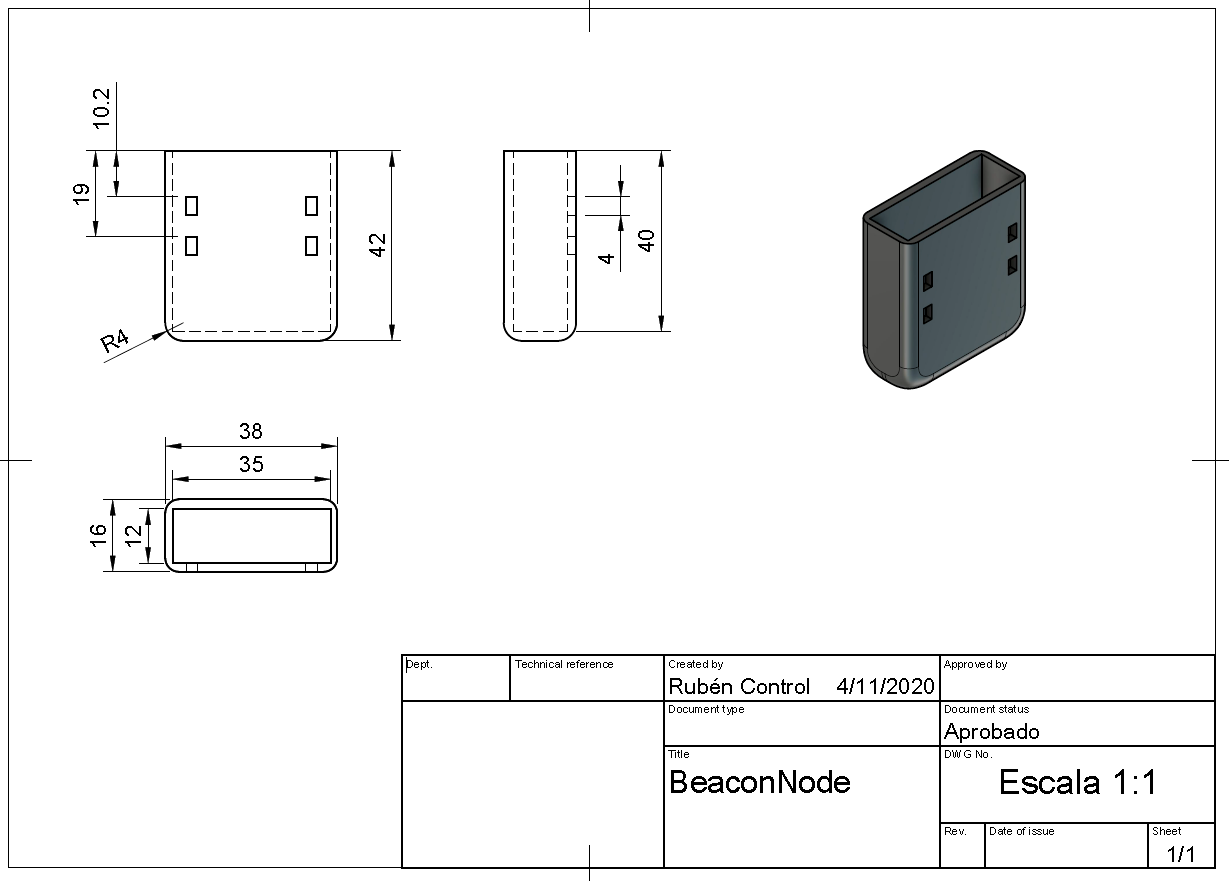
\includegraphics[width=0.6\textwidth]{../model_beacon.PNG}
                \caption{Plano y dimensiones del Beacon}
                \label{fig:mesh1}
            \end{figure}
        \end{center}
    \subsection{Imágenes de renderizado}
        Obtenemos el ensablaje desde el software CAD y en la figura 2 se muestra el renderizado del equipo.
        \begin{center}
            \begin{figure}[t]
                \centering
                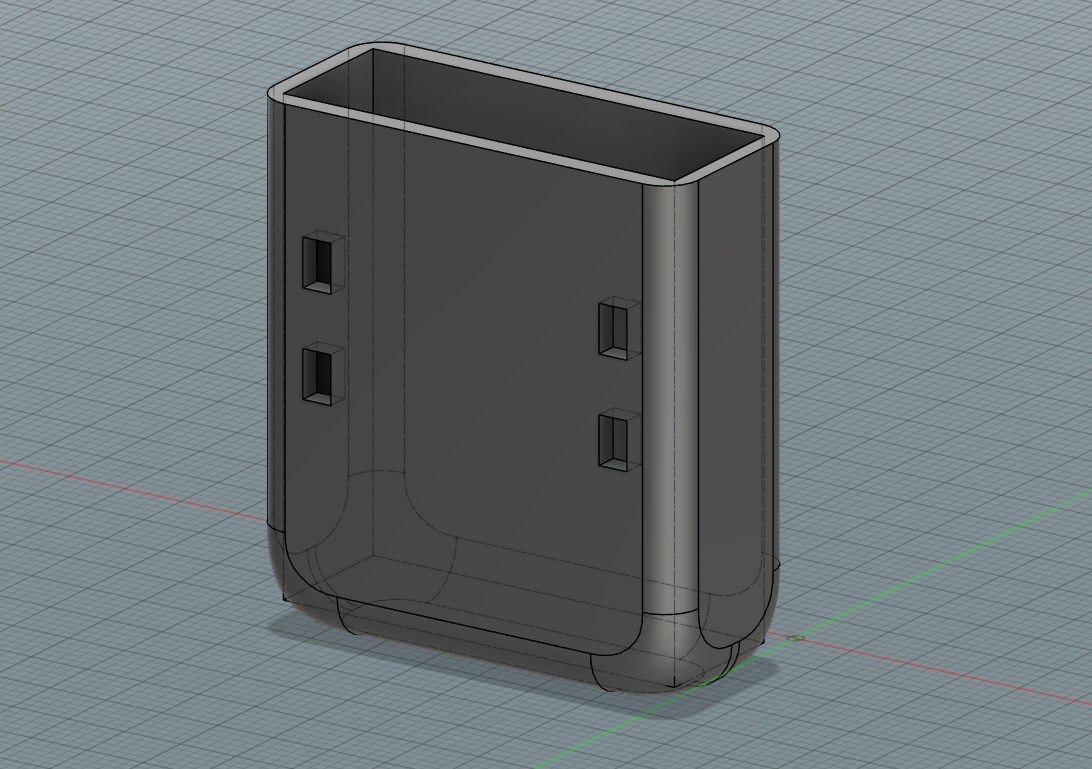
\includegraphics[width=0.3\textwidth]{../mechanical_beacon.PNG}
                \caption{Renderizado de la PCB}
                \label{fig:mesh1}
            \end{figure}
        \end{center}
    \subsection{Imágenes reales}
        Tras verificar el diseño en el ordenador se carga el filamento 3D y se procede a llevar a cabo la impresión, un par de horas más tarde
        se obtuvo la figura 3.
        \begin{center}
            \begin{figure}[ht]
                \centering
                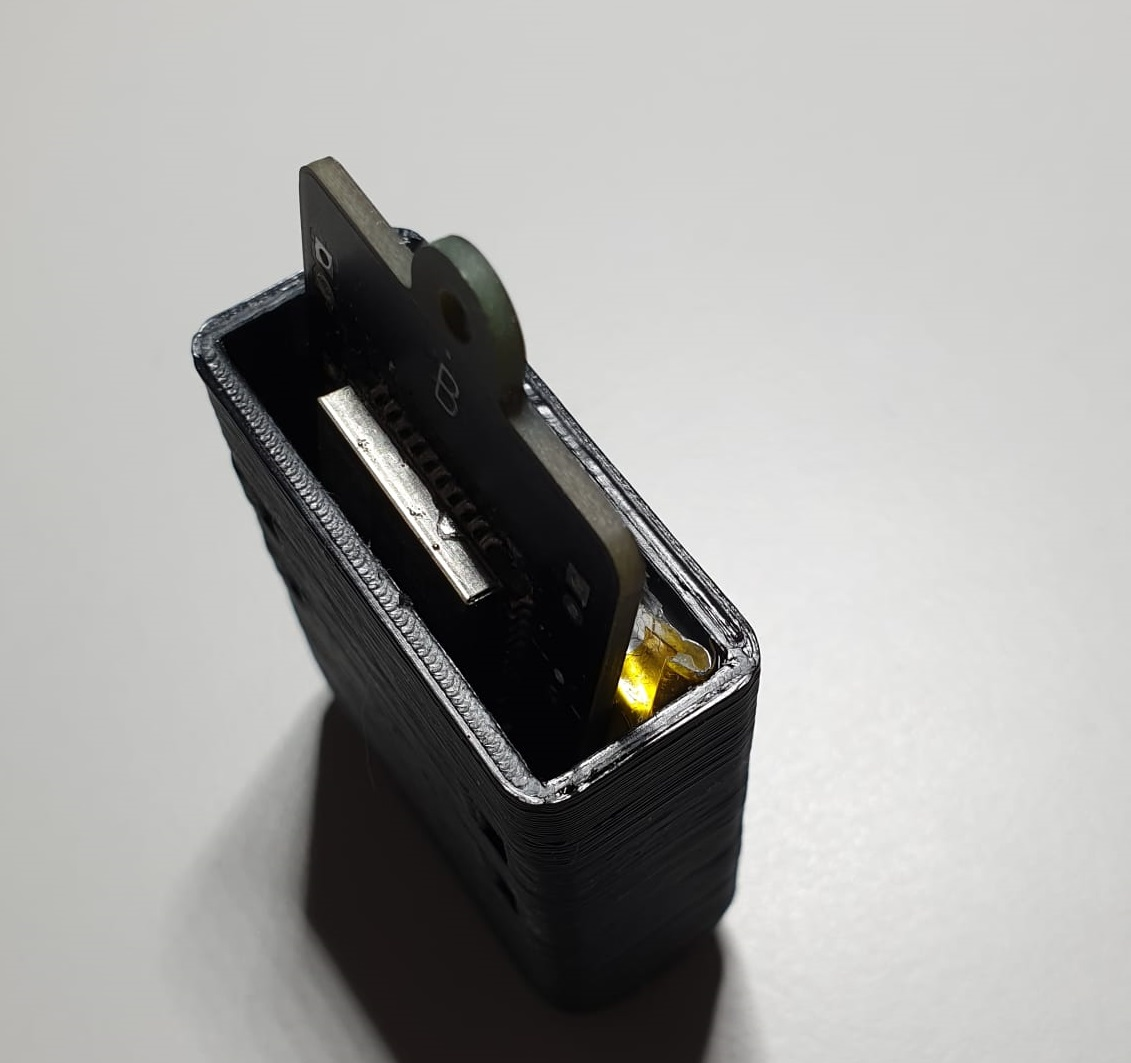
\includegraphics[width=0.36\textwidth]{../3d_beacon_1.jpeg}
                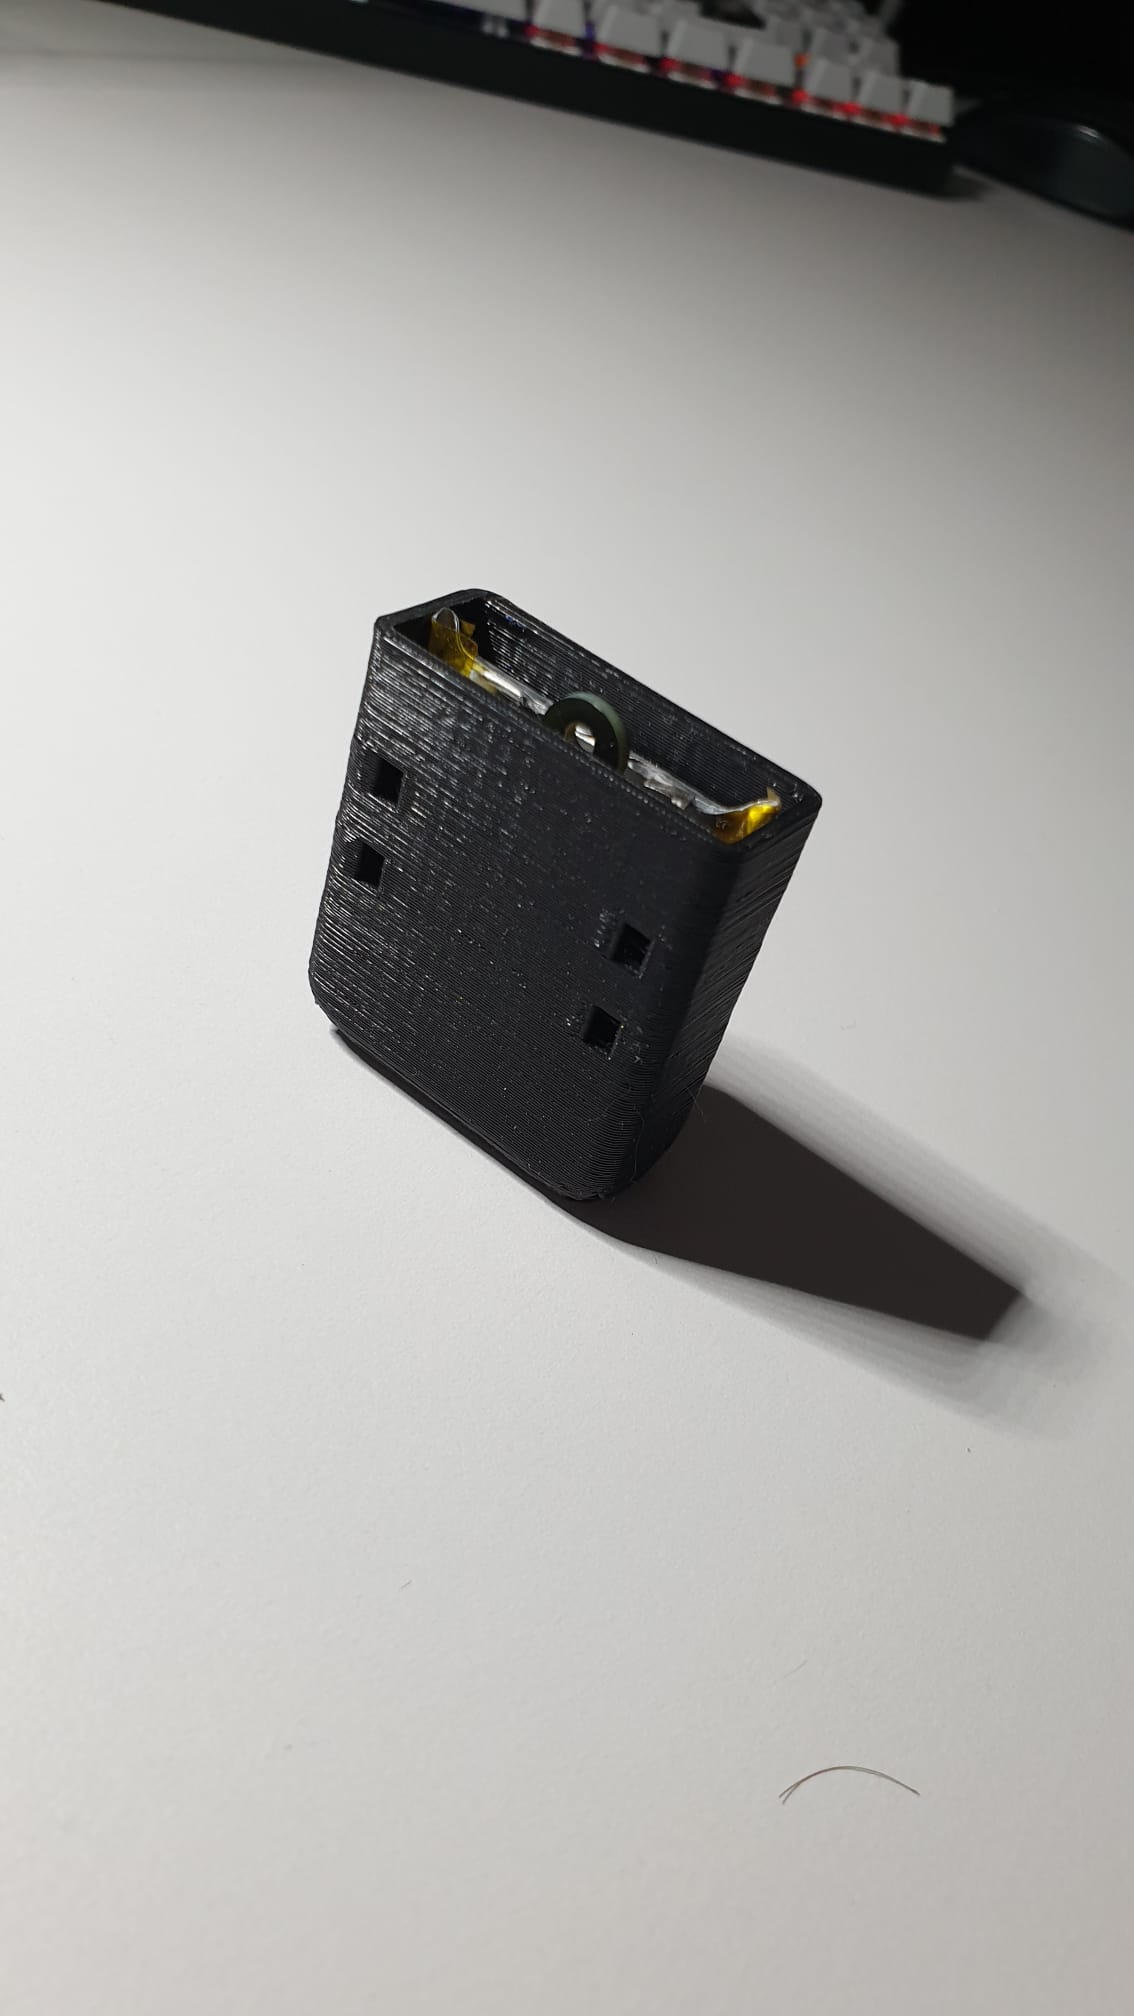
\includegraphics[width=0.4\textwidth]{../3d_beacon_2.jpeg}
                \caption{Imagen real del Beacon con batería.}
                \label{fig:mesh1}
            \end{figure}
        \end{center}

\section{Receptor Beacon o gateway}
    \subsection{Aspectos a considerar en el diseño}
        De nuevo se apuesta por reunir las especificaciones que ha de tener el contenedor de la electrónica:
        \begin{enumerate}
            \item Estéticamente atractivo, puesto que va a estar físicamente a la vista.
            \item Pequeñas dimensiones y discreto.
            \item Limitaciones en el tamaño de máximo 220x220x250 mm debido al volumen de impresión.
            \item Estructura sólida que garantize un buen agarre de la PCB en vertical.
        \end{enumerate}
        \paragraph{}
        Se ha de tener en cuenta que este equipo se encontrará en un lugar elevado atornillado o pegado a la pared, 
        es por ello por lo que se ha de hacer una caja robusta en la que no entre suciedad. 
    \subsection{Planos y dimensiones}
        \paragraph{}
        Partiendo de las dimensiones de la tarjeta, a continuación, en la figura 4, se
        muestran las medidas de la caja que lo alberga. 
        \begin{center}
            \begin{figure}[h]
                \centering
                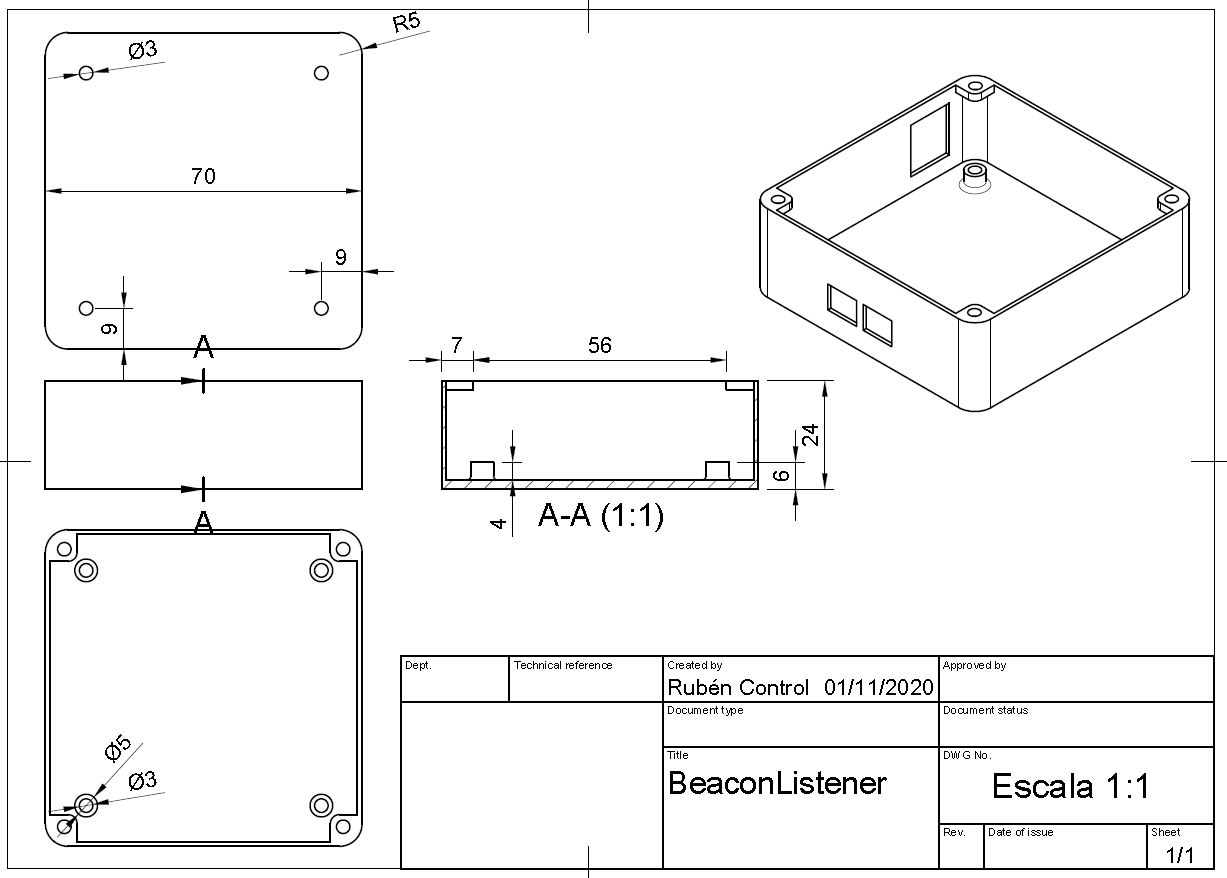
\includegraphics[width=0.55\textwidth]{../model_master.PNG}
                \caption{Plano de la caja del emisor.}
                \label{fig:mesh1}
            \end{figure}
        \end{center}
        \paragraph{}
        \paragraph{}

    \subsection{Imágenes de renderizado}
        Como se puede observar en la figura 5 se presentan los renderizados:
        \begin{center}
            \begin{figure}[h]
                \centering
                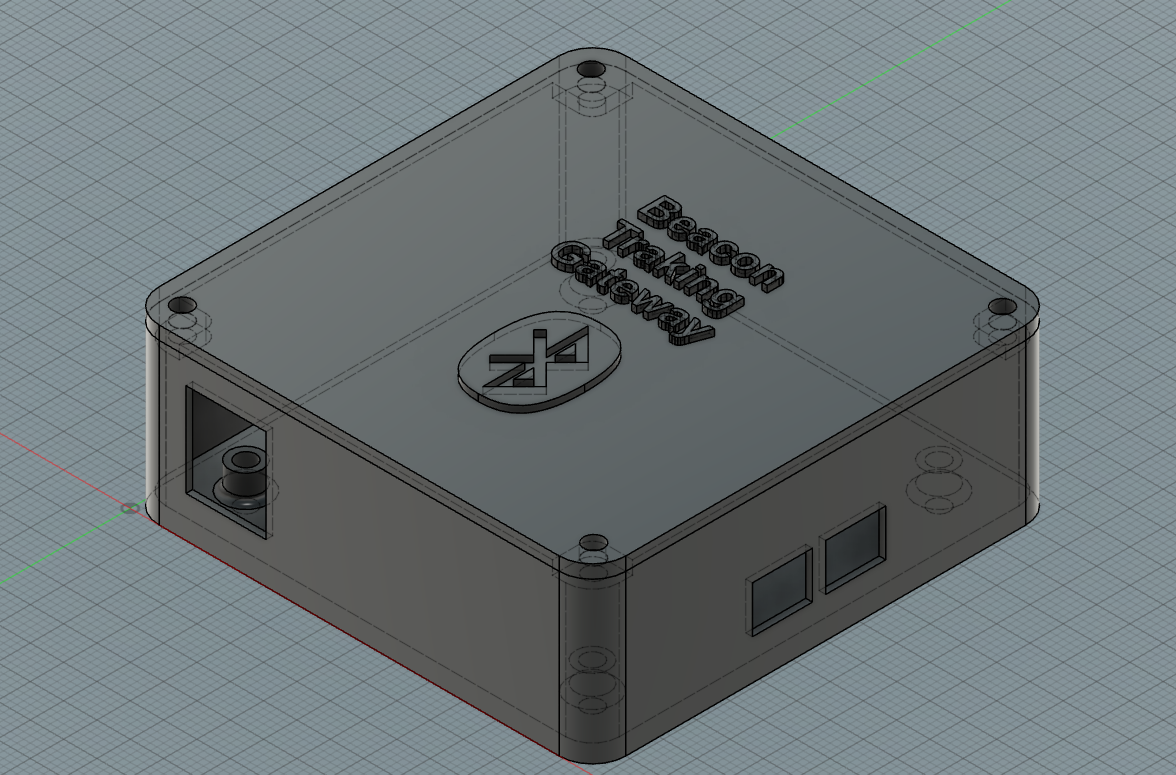
\includegraphics[width=0.55\textwidth]{../mechanical_master.PNG}
                \caption{Renderizado de la caja del emisor.}
                \label{fig:mesh1}
            \end{figure}
        \end{center}
        \paragraph{}

    \subsection{Imágenes reales}
        Una vez impresas las piezas y sin necesidad de lijar o ajustar algún apriete o tolerancia,
        el resultado es el que se expone en la figura 6.
        Introduciendo la electrónica dentro podemos ver el diseño completo en la figura 7.
        \begin{center}
            \begin{figure}[h]
                \centering
                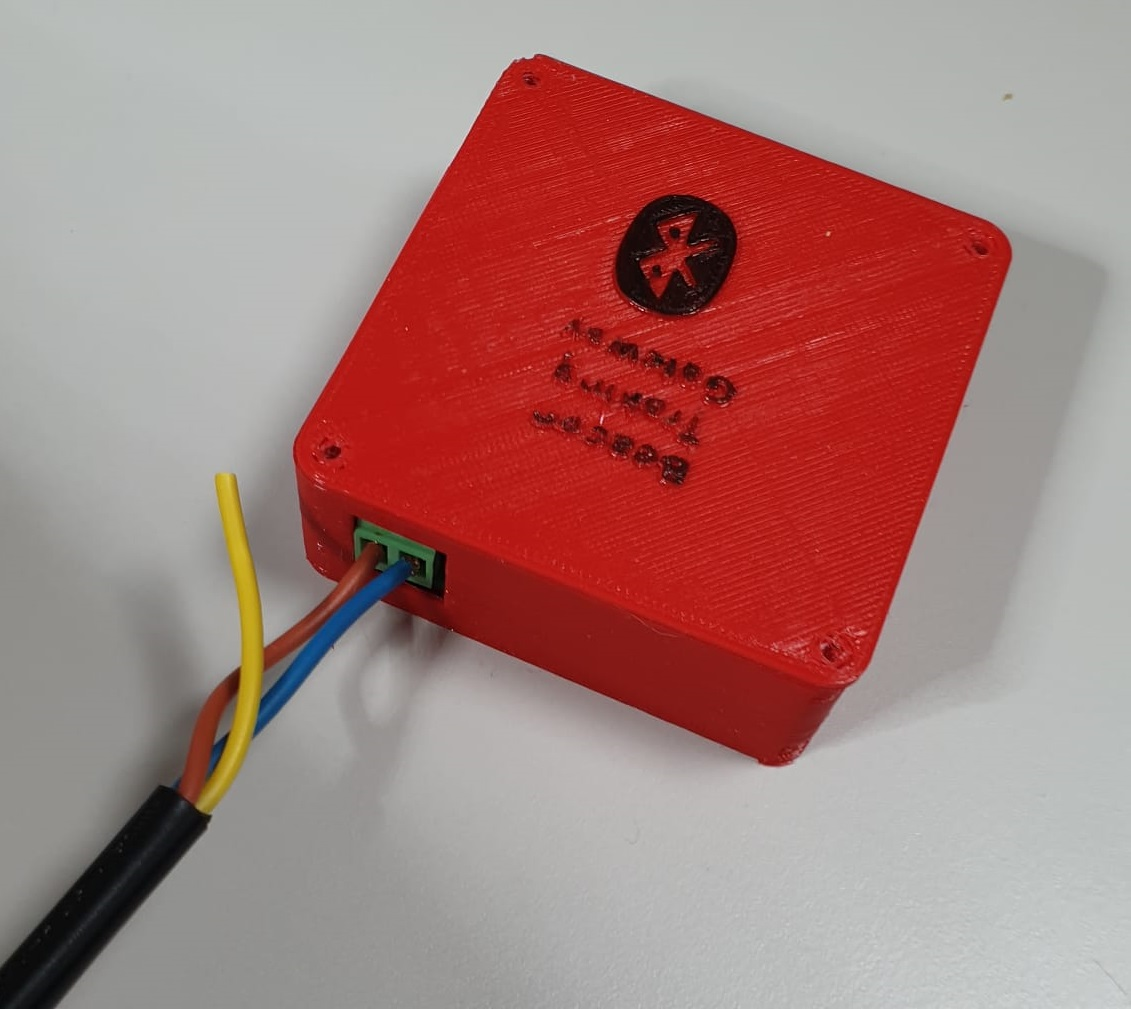
\includegraphics[width=0.3\textwidth]{../3d_master_1.jpeg}
                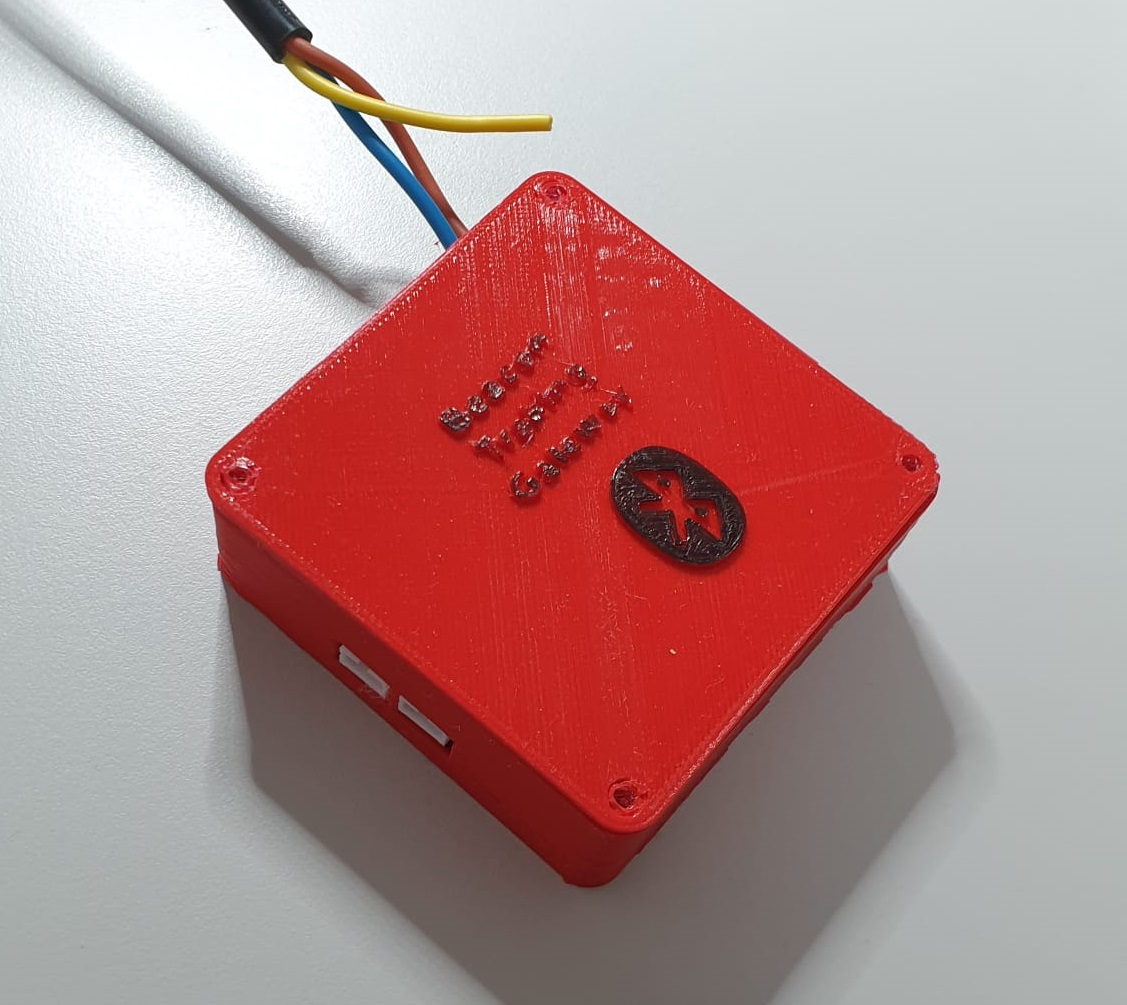
\includegraphics[width=0.3\textwidth]{../3d_master_2.jpeg}
                \caption{Caja real del receptor con dimensiones.}
                \label{fig:mesh1}
            \end{figure}
        \end{center}
        \paragraph{}
        \begin{center}
            \begin{figure}[h]
                \centering
                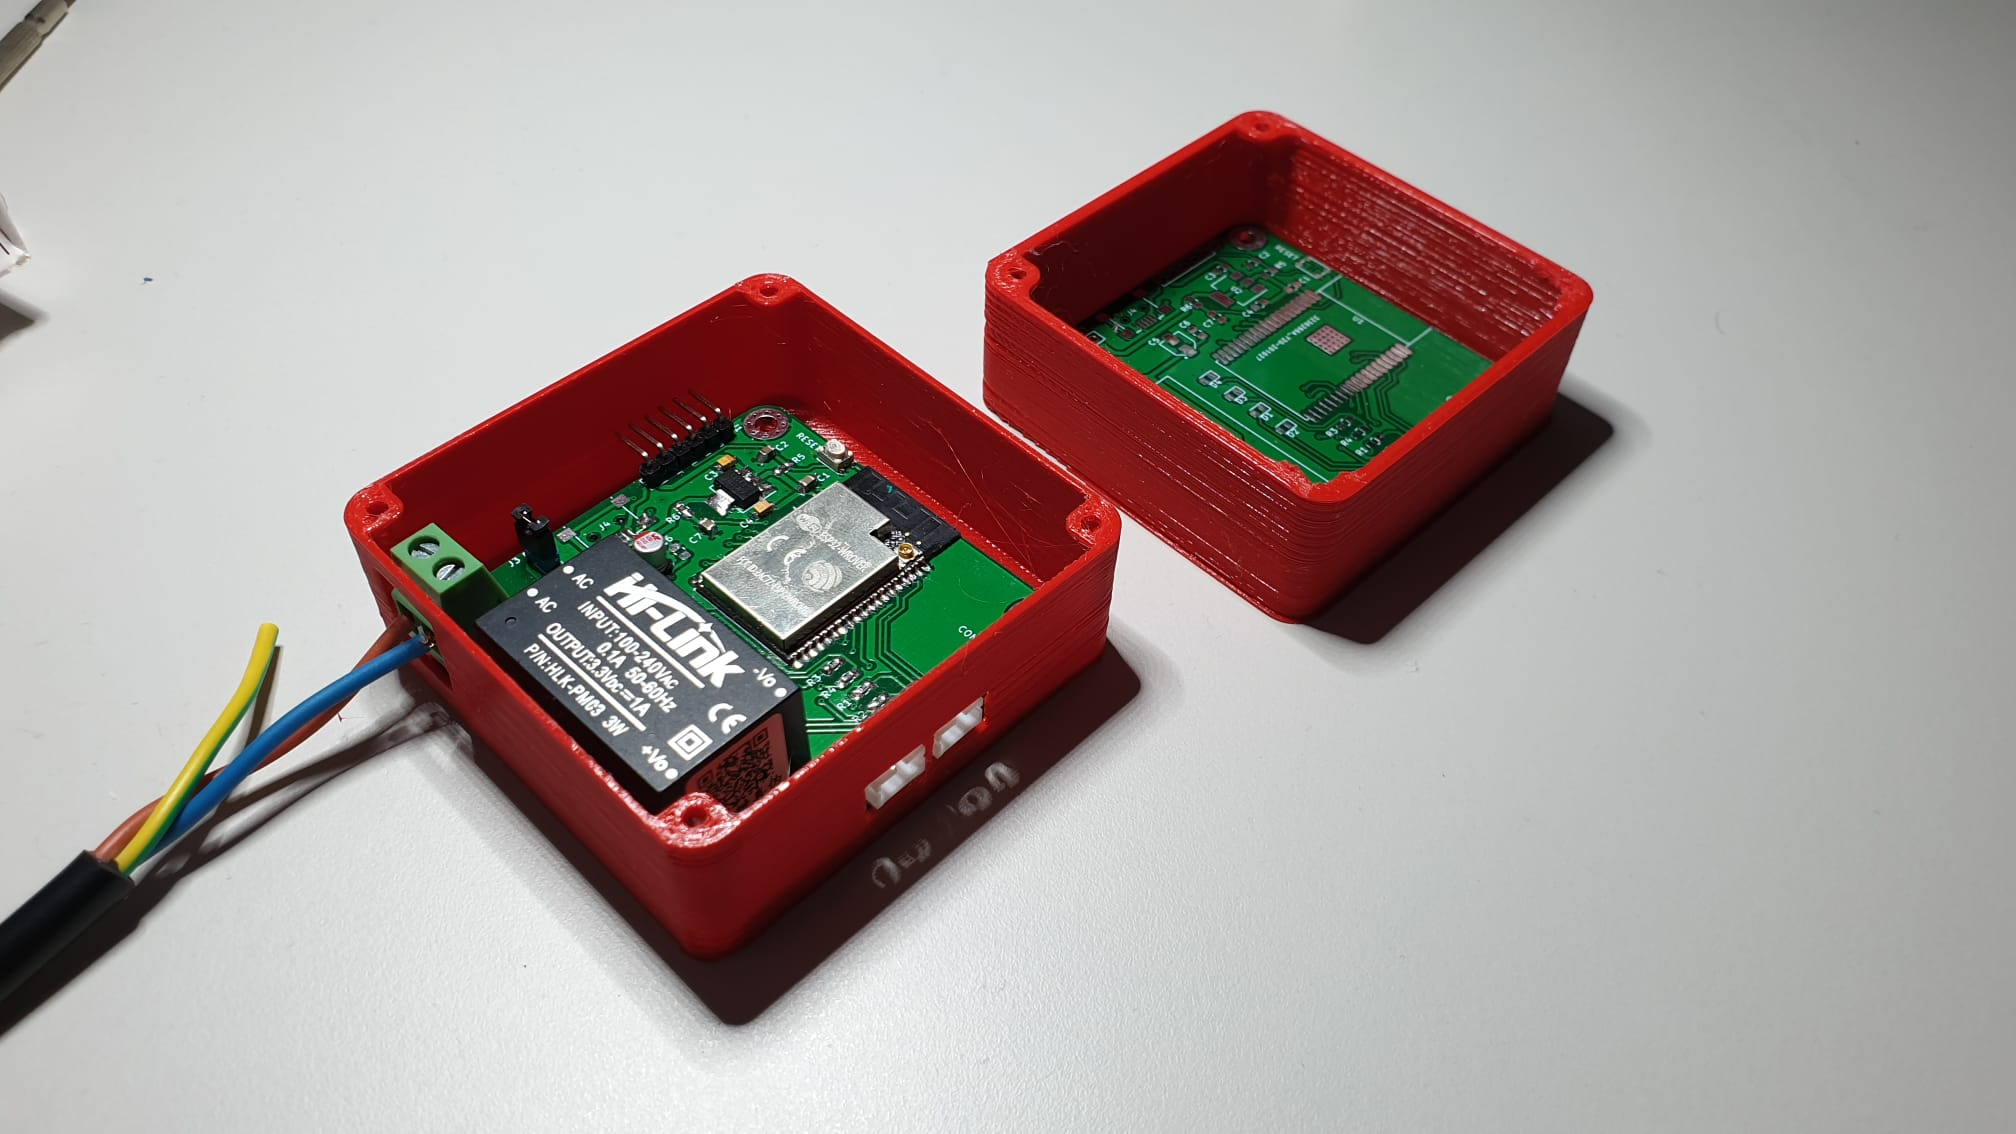
\includegraphics[width=0.58\textwidth]{../3d_master_2_box.jpeg}
                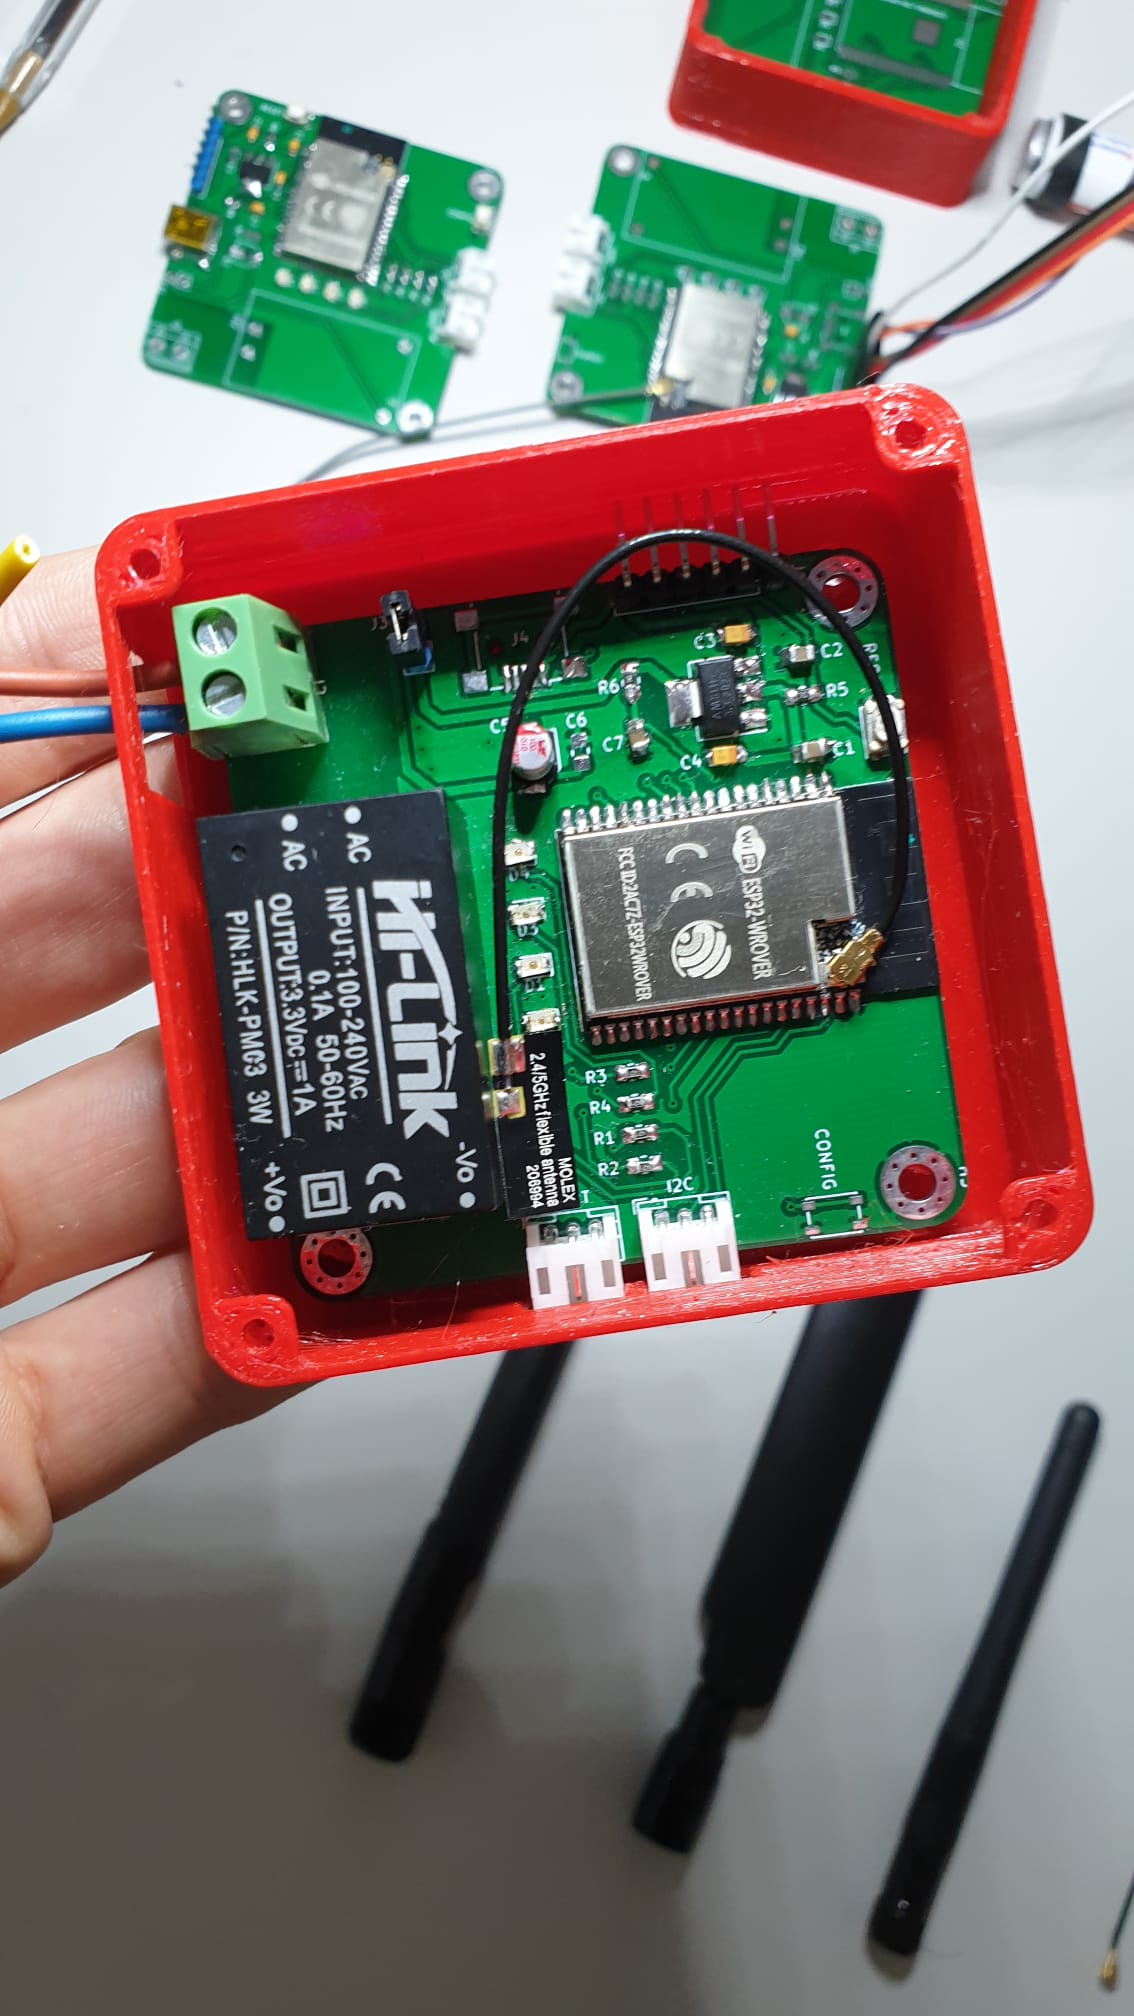
\includegraphics[width=0.4\textwidth]{../3d_antenna.jpeg}
                \caption{Caja real del receptor con electrónica dentro.}
                \label{fig:mesh1}
            \end{figure}    
        \end{center}
\section{Conclusiones}
    Tras desarrollar los primeros prototipos se procedió a llevar a cabo una prueba real con los mismos 
    en un entorno industrial para comprobar si era necesaria una versión 2.0 de los mismos, los resultados
    dejaron claro que este primer diseño era el acertado.

    Exceptuando una caída accidental, todos los diseños sobrevivieron a la prueba. Sin embargo, no se
    han podido tomar imágenes dentro de la planta, debido a las medidas de seguridad y a la ausencia
    de permisos por parte de la administración de la empresa.

    Igualmente los equipos de las fotos anteriores fueron los empleados y se aseguraron a unas estanterías con cinta de doble
    cara, con lo que se pudo hacer una una verificación del funcionamiento el firmware y una mejora del mismo.

\end{document}